\section{Lecture 30}
\begin{itemize}
    \item Steve $ \neq $ Diana
    \item Midterm \# M3-3116
    \item Covariance
    \item Correlation
\end{itemize}
If $ X $ and $ Y $ are independent:
\begin{align*}
    E(XY)&=
    \sum\limits_{x} \sum\limits_{y} x y f(x,y)\qquad\text{by defn}\\
    &= \sum\limits_{x} \sum\limits_{y} x y f
_X(x)f_Y(y)\\
    &=\sum\limits_{x} x f
_X(x) \sum\limits_{y} y f
_Y(y)\qquad\text{$ X,Y $ indep.}\\
    &=E[X]E[Y]
\end{align*}
$ \implies Cov(X,Y)=E[XY]-E[X]E[Y] $. Thus, $ X,Y $ independent
$ \implies Cov(X,Y)=0 $, but $ Cov(X,Y) = 0 $ \myuline{does not}
mean $ X,Y $ are independent.

Uncorrelated variables \myuline{could} still be dependent. If, for
instance there is a non-linear relationship.

\begin{center}
    
\includegraphics{covnot0.png}
\end{center}

\myuline{Other points about covariance}:
\begin{itemize}
    \item if $ Cov>0 $, then $ X\uparrow \iff Y\uparrow $ OR
    $ X\downarrow \iff Y\downarrow $.
    \item if $ Cov<0 $, then $ X\downarrow \iff Y\uparrow $ OR
    $ X\uparrow \iff Y\downarrow $.
    \item the magnitude of $ Cov(X,Y) $ can't be interpreted. We need
    to rescale to a restricted range to interpret size.
\end{itemize}

\myuline{Correlation}
\begin{defbox}
    \subsection{Definition (Correlation Coefficient)}
    The \emph{correlation coefficient} $ \rho_{x y} $ of $ X $ and $ Y $ is:
    \[ Corr(X,Y)=\frac{Cov(X,Y)}{\sqrt{Var(X)}\sqrt{Var(Y)}} \]
    \[ \rho=\frac{\sigma_{x y}}{\sigma_x\sigma_y}  \]    
\end{defbox}

\myuline{Notes}
\begin{itemize}
    \item sign of $Corr$ = sign of $Cov$ for any given $ X,Y $.
    \item $ -1\le\rho_{x y}\le 1 $ (see course notes)
    \item only equal to $ \pm 1 $ if $ Y=aX+b $
\end{itemize}
We interpret the magnitude of the correlation as the \myuline{strength}
of the linear relationship.

\begin{center}
    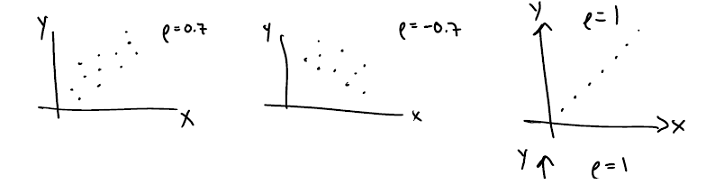
\includegraphics{correlation.png}
\end{center}

\textbf{Important}: correlation \myuline{does not} imply causation!

if $ \rho=0.95 $, then
\[ \begin{cases}
    X \text{ causes } Y \text{ OR }\\
    Y \text{ causes } X \text{ OR }\\
    X,Y \text{ are caused by } Z\\
    X,Y \text{ are correlated by chance}\\
\end{cases} \]

\myuline{Example}

(from past lecture)

Suppose $ X= $ \# apple products and $ Y= $ \# Microsoft products (given at least
one of each) have a joint pf:

\begin{tabular}{| *{4}{>{\centering\arraybackslash}p{2cm} |}}
    \hline
    $y\backslash x$ & 1    & 2    & 3    \\
    \hline
    $1$             & 0.30  & 0.17 & 0.20 \\
    \hline
    $2$             & 0.17 & 0.10  & 0.06 \\
    \hline
\end{tabular}

$ Cov(X,Y)=-0.0407 $

$ Var(X)=E(X^2)-1.79^2=0.6859 $

$ Var(Y)=E(Y^2)-1.33^2=0.2211 $

$ Corr(X,Y)=\frac{-0.0407}{\sqrt{0.6959}\sqrt{0.2211}}=-0.1045 $ ... a weak
negative correlation.

\myuline{Example}

Roll a fair $6$-sided die $ 10 $ times.
$ X_1= $ \# 1's
$ X_2= $ \# even composites (4,6)

$ Cov(X_1,X_2)=5-\nicefrac{10}{6}\times \nicefrac{10}{3}=-0.556 $

$ Var(X_1)=10\left( \nicefrac{1}{6} \right)\left( \nicefrac{5}{6} \right)=1.389 $ ($ npq $)

$ Var(X_2)=10\left( \nicefrac{1}{3} \right)\left( \nicefrac{2}{3} \right)=2.222 $ ($ npq $)

$ Corr(X,Y)=\frac{-0.556}{\sqrt{1.389}\sqrt{2.222}}=-0.316 $

\myuline{Next class}: Linear Combinations of Random Variables